\documentclass{article}
\usepackage{graphicx} % Required for inserting images

\title{Analysis of research and media for air quality and health data: A South Africa, Kenya, and UK Comparison}
\author{Karega Pauline}

\begin{document}

\maketitle

\section{Introduction}

Since the beginning of urbanization, there has been a significant decline in global ambient air quality. Anthropogenic activities have disrupted natural ecosystems, leading to changes in the atmosphere that, in turn, impact human health (Mukherjee and Agrawal, 2018). Air quality has therefore become a crucial area of research due to its profound effects on public health. Research has linked poor air quality to respiratory diseases (Bi et al., 2023; Glick et al., 2019; Kravitz-Wirtz et al., 2018), cardiovascular diseases (Basith et al., 2022), and neurological development issues, and cognitive decline, especially in children (P. N. deSouza et al., 2022; Ha, 2021), and the premature deaths of millions per year (Goldsborough et al., 2023; Yu et al., 2024). 

While the burden of air pollution is a global concern, its distribution, causes, and mitigation capacity differ sharply between high-income and low- to middle-income regions (Jabareen, 2023). In the global South, natural phenomena, industrial expansion, rural-urban migration, increased traffic emissions, and reliance on biomass for heating and fuel are leading sources of emissions, and most countries register pollutant levels exceeding those suggested by the WHO (Kutlar Joss et al., 2017). In contrast, in the Global North, greenhouse gas, traffic, and industrial emissions form the main contributors of pollutants. Global North countries list pollution levels less than those suggested by the WHO (Ngui et al., 2016). While the general knowledge of air pollution status is known globally, the understanding of pollutant types, nature, and levels varies in these regions due to the availability of resources used to measure emissions, policies to mitigate anthropogenic practices that contribute to pollutants, and the agencies and governments responsible for monitoring these policies. 

To address the issue or provide a clear picture of what is happening, reliable data sources are needed that encompass both health and environmental data. These sectors have been well established in the Global North for years, compared to the Global South. In fact, in multiple countries of the Global South, the majority of the air quality and health sector heavily depends on funding from the West. Additionally, data practices in the Global North and South differ, which influences how data moves through the data pipeline and research, and creates varying barriers to data use. These barriers in the data pipeline in both settings must be adequately understood to address the existing gap in research between the regions and provide potential solutions. 

A comparative review of literature and the media offers a glimpse into the data journeys of researchers as they strive for data-driven insights into the impact of air quality on health and policy. Investigating the data collection methods, data sources, data storage, and sharing can provide insight into the technical barriers faced by researchers as they attempt to utilize this data. Further qualitative work can also provide us with the assumptions and beliefs that accompany the technical barriers in the same pipelines. As such, we will be able to make adequate comparisons between the regions of interest to offer solutions.    

\section{Literature Review}

Proper data governance is key for data-driven ventures, including research and policymaking. Clear guidelines for the collection, access, storage, sharing, and ownership of every dataset used in research are necessary. Data governance, however, has proven to be a challenging area in multiple sectors, including environmental and health research. There needs to be a straightforward way to search for and access data for various stakeholders throughout the data life cycle.   

The impact of air quality on human health is a significant global concern, with air pollution contributing to up to seven million premature deaths worldwide \cite{fuller_pollution_2022}. While the burden of air pollution is a worldwide concern, its distribution, causes, and mitigation capacity differ sharply between high-income and low- to middle-income regions \cite{jabareen_increasing_2023}. In the global South, natural phenomena, industrial expansion, rural-urban migration, increased traffic emissions, and reliance on biomass for heating and fuel are leading sources of emissions, and most countries register pollutant levels exceeding those suggested by the WHO \cite{kutlar_joss_time_2017}. In contrast, in the Global North, greenhouse gas, traffic, and industrial emissions form the main contributors of pollutants. Global North countries list pollution levels less than those suggested by the WHO \cite{ngui_kenyas_2016}. While the general knowledge of air pollution status is known globally, the understanding of pollutant types, nature, and levels varies in these regions due to the availability of resources used to measure emissions, policies to mitigate anthropogenic practices that contribute to pollutants, and the agencies and governments responsible for monitoring these policies.

Many countries in the Global South prioritize other concerns, such as infectious diseases, and therefore do not prioritize issues like air quality and health. However, with multiple of these diseases having been addressed, the research focus is shifting to issues like climate change and health, and more specifically air pollution and health \cite{fuller_pollution_2022}.  

To develop effective policies and ensure air quality is suitable for human health, there needs to be relevant and accurate data. To ensure adequate data availability, we explore the pollution profiles of our areas of interest and compare to the available data and their impact on health.

\subsection{Kenya} 
Kenya, has a diverse and region-specific pollution profile influenced by varying sources across the country. In major urban centers such as Nairobi and Mombasa, air pollution is predominantly driven by traffic congestion, road dust, and vehicular emissions \cite{singh_urban_2022}. Additionally, the majority of the vehicles are second-hand, and the fuels are sulfur-based contributing to pollutants like black carbon, Sulfur dioxide, organic compounds, green house gases like short lived climate pollutants \cite{mbandi_assessment_2023}. The reliance of informal settlements on biomass fuel also significantly contributes to degraded air quality in major cities, especially indoor air quality \cite{noauthor_analysis_nodate}. In contrast, smaller towns and rural communities experience pollution from agricultural practices, including the use of fertilizers and pesticides, as well as emissions from small-scale mining operations. Along the coastal region, particularly near port cities like Mombasa, maritime activities contribute significantly to air pollution through emissions from ships, cargo handling, and industrial activities related to shipping and logistics \cite{ogara_understanding_2025}. 

Air quality monitoring in Kenya is primarily conducted using a combination of ground-based monitoring stations and low-cost sensor networks \cite{oguge_fine_2024, pope_airborne_2018}. These systems provide real-time and localized data but are limited in coverage and precision. Pollutants primarily monitored are particulate matter PM2.5 and PM10. Gaseous pollutants are rarely measured due to the lack of instrumentation. The national government, which is responsible for the ground-based monitoring stations, also lacks a centralized data access point for environmental data. Local county governments own low-cost sensors distributed across counties, but also lack central data access points. These low-cost sensors, heavily relied on in Kenya, have low spatial resolution. Additionally, the accuracy of the data is questionable due to the lack of proper calibration of these instruments \cite{tekouabou_towards_2022}. This poor cohesion in government also results in sparse or entirely lacking data from other regions, except for Nairobi, and a few hot spots. This results in significant gaps in national air quality assessments, hindering the development of targeted policy interventions.

In addition, cohort-based studies have been conducted to collect data on indoor air quality, particularly in densely populated residential areas, to gain a more comprehensive understanding of human exposure. However, most of these projects are institution-based and funded by external institutions, and their data are not made available for public use \cite{desouza_air_2020}.  

Non-governmental organizations (NGOs), and individuals also play a crucial role in data collection in Kenya, with personal air quality monitors \cite{singh_urban_2022}. However, their contribution is difficult to quantify due to their lack of visibility. Additionally, the lack of expertise in such initiatives results in unreliable air quality data \cite{pinder_opportunities_2019}.  

Health data collection in Kenya remains fragmented and largely paper-based, particularly outside of large hospitals \cite{karuri_dhis2_2014}. The Government of Kenya has deployed various health information systems across the country, including laboratory information systems (LIS), the Kenya Health Information System (KHIS), and the Kenya Health and Research Observatory (KHRO), among others \cite{yetu_electronic_nodate}. Kenya also has a national insurance fund, (NHIF), recently changed to the social health insurance fund (SHIF), under different management \cite{barasa_kenya_2018}. The majority of this data is used for staffing, commodity supplies for community health programs, and patient management. They are rarely used for health research or other interdisciplinary studies due to their inaccessibility and format. The spatiotemporal information documented for each patient may not be helpful for exposure analysis. Additionally, the healthcare space is filled with local, small-scale clinics and private providers, who have bespoke data management systems, which hinder comprehensive health surveillance and accelerate data fragmentation \cite{mwangi_accessibility_2014}. The lack of centralized management and access makes it difficult to achieve interoperability.

Therefore, exposure assessment heavily relies on longitudinal cohort studies and mortality or statistical health reports from platforms such as the Kenya National Bureau of Statistics. However, these are often patchy and delayed. Additionally, the Global Burden of Disease (GBD) serves as a reliable source of information; however, in some country-specific cases, including Kenya, it often contains outdated or incomplete records \cite{noauthor_global_nodate}. 

Data availability has been proven not to be an issue in Kenya. Multiple data sources exist. However, the available information or narrative does not align with the available data. The Kenyan research space has been vocal about helicopter science. Therefore, the air quality and health research space may also be marred by the same issues: siloed data collection and research, informal workflows, hesitant data sharing practices, and more. An investigation into the technical and social factors that contribute to this disparity is needed.    
 

\subsection{South Africa}

Compared to Kenya, South Africa presents a distinct yet complementary case in this study. As one of the most industrialized and urbanized economies on the continent, its historical development has been shaped by mining, agriculture, and a diverse manufacturing sector. South Africa’s major cities—such as Johannesburg, Cape Town, and Durban—are densely populated and face complex, city-specific air quality challenges. These include industrial emissions, high vehicle traffic, and seasonal weather conditions such as wintertime air stagnation \cite{liebenberg-enslin_air_2024}. Coal-powered power plants make up the major pollutant contributors in many regions, and individual diesel-powered generators help combat electricity issues in private residences \cite{wright_impact_2024, makoni_coal-fired_2023}. 

Primary pollutants include particulate matter, NO2, and SO2. Regional studies also focus on radon pollution from mining fields \cite{mphaga_radon_2024}. The region also needs to consider pollutants transported across its borders by transboundary air, especially of NO2, and SO2 \cite{matandirotya_spatiotemporal_2021}. However, monitoring infrastructure remains uneven, and many urban and peri-urban areas lack sufficient sensors to provide continuous and high-resolution air quality data \cite{liebenberg-enslin_air_2024}. Unlike Kenya, however, South Africa has the SAAQIS (South African Air Quality Information System) database, which provides data on multiple pollutants nationwide. The data is sourced from ground monitoring stations managed by the governments. This data, however, is quite fragmented, missing days and months of readings for different stations and regions. This limits the ability to create a straightforward, data-driven narrative of environmental exposure and health risk across the country.

Additionally, similar to Kenya, individuals and NGOs also play a crucial role in contributing data and communicating results through public engagement. They fill in for the government where it is lacking \cite{najar_challenges_2025}. This contribution by such groups, however, complicates data availability or accessibility due to their lack of proper expertise to contribute to the data lifecycle.

On the health side, South Africa, like other African countries, has been adapting to the digitization of their health records \cite{katurura_electronic_2018}. The National Department of Health coordinates national health strategy and oversight, while the South African Medical Research Council (SAMRC) plays a leading role in health research and innovation. SAMRC’s focus spans both communicable diseases—such as HIV/AIDS and tuberculosis—and an increasing concern with non-communicable conditions, particularly maternal, neonatal, and chronic illnesses. These records are, however, collected for the purpose of monitoring patient outcomes, managing the performance of providers, and tracking the use of public funds and resources \cite{conco_accessing_2025}. The data is not collected or used for health research. The central government is also establishing a national health insurance scheme aimed at improving accessibility to health, which has the potential to serve as a valuable research resource. However, the implementation of these systems and the overall goal of interoperability are hindered by a lack of proper infrastructure, inadequate government support, and resistance from healthcare workers \cite{wright_electronic_2017}. 

Multiple evidence scenarios demonstrate the crucial importance of understanding the factors that lead to the disconnect in data flow systems in health and environmental data integration in South Africa, despite the availability of resources. South Africa is listed as having the highest prevalence of childhood asthma; however, cohort studies cannot provide the full extent of the issue, and the lack of access to health data makes it difficult to establish the association between the asthma cases and the environmental source. The Highveld Priority Area Project was launched in 2007, and its failure a decade and a half later highlights the need to address the presenting issues in the workflow. 


\subsection{UK}
Compared to Kenya and South Africa, the UK presents a more established region with a well-established air quality and health research network, featuring advanced air quality monitoring systems that include ground-based air quality monitors and more centralized data access points \cite{noauthor_defra_nodate}. Pollution contributors include pollen, road traffic, industries, and more. For air quality data, the UK government and environmental agencies provide data from functional weather monitoring stations across the UK \cite{noauthor_air_2025}. Centralized data sources such as the Met Office, DEFRA, Copernicus, CEDA, TROPOMI, and more. These sources feed into each other to form a cohesive data source. The database provides data on particulate matter, gaseous pollutants, and ozone. The Met Office also provides pollen data.              

For health, the United Kingdom has multiple data sources as well—electronic health records, open prescription data, statistical data, and synthetic data. The UK, through services like Health Data Research UK and trusted research environments, is making electronic health records traditionally collected for patient care and resource distribution available for use in research \cite{sebire_hdr_2020}. Given the sensitive nature of the data, however, data access is quite a challenge. The usability of the data has also been questioned. 

Policies are data driven decisions. Or at least they should be. In the research or data lifecycle, these consequences of the data analysis, i.e policies, are usually published in the media, and are usually the level at which the public engage with the data. This creates a cycle of engagement both within and outside the research space resulting in addition of actors in the data space. 

In terms of air quality and health, the topic is of importance to multiple sectors or industries. These include transportation industry, environmental agencies, NGOs, and more. As such, they use data in their work and missions. And they publish websites, articles, reports and more. And as evidenced by publications, reports, and policies churned out each year, it attests to the availability of data, in multiple formats or at different levels of accessibility. We can therefore trace the data journeys from these, having a glimpse at data collection methods available, challenges encountered, and solutions. These can be used to look into available resources and further infer barriers and challenges to health and environmental data linkage.     

The media plays a crucial role in communicating the impact of air quality on health. In the data life cycle, it plays a vital role in shaping public understanding and stakeholder priorities. It is used to communicate the results of analysis in the form of policy recommendations, the impact of policies, or to raise concerns where focus should be redirected. Its role in communicating the results of data analysis, such as policies, is well known. Its role in communicating about the earlier parts of the data life cycle and further highlighting additional socio-technical issues in the pipeline, is however overlooked. In Kenya, for example, data users outside the research community receive news about mobile air quality data collectors and monitors placed in the city from the media first, rather than institutional websites. In South Africa, additional data collected by environmental agencies separate from the government and research organizations use the media to communicate about their data. For regions where data is fragmented and lacking, the contribution of all stakeholders involved would fill in data gaps.

We can use these to find stakeholders outside the traditional health and environmental research path, and find other data providers or platforms that they use to produce the policies. Or infer their interaction with others in the data lifecycle, toward building these policies.  

   

\section{Problem Statement}
In many low- and middle-income countries, including Kenya and South Africa, environmental and health data are generated and governed by different systems, institutions, and practices. Despite growing recognition of the need to link these data to address complex challenges—such as the health impacts of air pollution- efforts to do so remain fragmented, inconsistent, or limited in scope. This fragmentation is not only technical but also deeply socio-technical, involving issues of data ownership, institutional silos, informal workflows, underdeveloped infrastructure, and limited policy translation. While air pollution data may be available from environmental agencies, and health data from ministries or hospitals, the systems through which they are collected, managed, and used are rarely coordinated. The result is a gap in evidence-informed policymaking, particularly in under-resourced settings where the burden of disease and exposure to environmental risk are highest.

Furthermore, existing research often focuses on either technical or policy dimensions in isolation, with limited attention to the lived realities, institutional cultures, and social assumptions that shape how data is collected, interpreted, and shared. There is a critical need to understand these socio-technical dynamics in practice to inform more integrated, usable, and equitable data systems. Our three regions of focus have different levels of maturity in the fields, and a comparison can offer insights into how their data practices and dynamics differ. 


Our objectives were:
1. Evaluate air quality and health related media especially news articles, policy documents, and research publications to obtain their data pathways.


2. Infer the major stakeholders within and without the research pathway and their contribution to the data lifecycle.


Generally, we aimed to work backwards from points of policy, and public engagement, to trace their work with data, or engagement with other data stakeholders, to see how the data flowed to be able to inform all the practice.

To achieve these objectives, the proposed methodology is as follows.

\section{Methods}

1. Article search for the media's contribution of data

We use Feedparser v6.0.11 to scrape news feed data. Feedparser is used to download and parse feeds. We obtained news articles about air quality and health in Kenya, South Africa, and the United Kingdom. We targeted media houses that offered both digital and print articles. For Kenya, we used Nation Africa, Standard Media, and The Star. South Africa, Daily Maverick, timeslive, and news24. And for the UK, BBC, The Guardian, and The Telegraph. We did not specify any timelines and gathered all articles, with our code stopping at a maximum of 1500 articles. Our search terms were as follows: "air pollution", "air quality", "climate change", "respiratory illness", "respiratory diseases", and "pollution policy". 

We excluded articles whose context was air quality and health-related, but from other countries. For example, multiple UK articles addressed wildfires in Canada, and how those impacted air quality. 

These search terms informed our categorization of the articles based on key topics that generally addressed air quality and health in the different countries. These were as follows; Air Pollution and Quality'. 'health', 'disease', 'illness', 'mortality', 'asthma', 'dementia', 'respiratory', returned 'Health and Disease Impact'. 'climate change', 'global warming', 'emissions', 'weather', 'heatwave', returned 'Climate and Environment'. 'vehicle', 'transport', 'bus', 'boda', 'ulez', 'clean air zone' returned 'Transport and Mobility'. 'fuel', 'stove', 'cooking', 'industry', 'factory', 'factories', 'mining', 'energy' returned 'Energy and Industry'. And, 'waste', 'burning', 'landfill', 'recycling', 'deforestation', 'land use', returned 'Waste and Land Management'. 

2. Analysis of data used in published articles in Kenya and South Africa on air quality and health. 

We searched PubMed and Crossref for publications using key words "air pollution", "air quality", "pm2.5", "pm10", "CO", "NO2", "particulate matter", "emissions", for air quality, and "health", "COPD", "respiratory", "asthma", "mortality", "morbidity", "disease", "hospital", for health.

The publications had to make mention of the data used, therefore, data source, and format. A clear path of data collection, storage, transfer had to be there. 
We also excluded purely qualitative studies.

3. Policy document mining and going through the text about the data used to make these policies.


4. Qualitative data collection through interviews and focus groups. Following ethical approval, we have set up interviews and focus groups with individuals and institutions that form major stakeholders in the air quality and health sectors, to gather information about their data journeys. These include non-governmental organizations that collect data for public empowerment, an end-to-end business that installs sensors on behalf of the county government, county government data professionals, a private policymaking organization working with the government to create air quality policies, and hospitals to investigate their data collection and use with environmental data. 

\section{Results}

\subsection{Media analysis of key stakeholders, and data used in public communication}

This section examines how the media presents information about air quality and health in the three regions, including mentions of pollutants, data availability used to generate the reports, health information, and policies. It also examines the authorities or stakeholders responsible for presenting information and their data usage. 
The data used for this section was collected using web scraping of news articles and sites, conference websites and presentations, data provider sites, and public surveys issued by government and non-government groups. We also use published articles on the subject. 



\subsection{Analysis of data used in published articles in Kenya and South Africa on air quality and health} 

Inclusion criteria
We restricted our search to PubMed and obtained 138 records from South Africa, 51 publications in Kenya, and 965 in the UK. This was without a time restriction, and due to volume we reduced them to cover publications from 2010. This was due to 
We included articles that mentioned the country, specific towns within each country, and where the country in question was a key part of the study and had separate data from each even among the whole dataset.

Exclusion Criteria



\section{Results}

\subsection{Grey literature analysis for air quality and health data}

Despite the disparity in timelines, with the UK having a decade's head start on Kenya and South Africa, we observe a general upward trend in air quality and health publications. Initially, the issue was presented under the generalized climate change umbrella. However, we have seen a more focused approach over the past decade in all regions. This speaks to the increasing importance of the issue, and general visibility and interest among the general public. 

There was a general spike in articles from 2020, which can be linked to COVID-19 and the effects that the restrictions had on the environment.

\begin{figure}
    \centering
    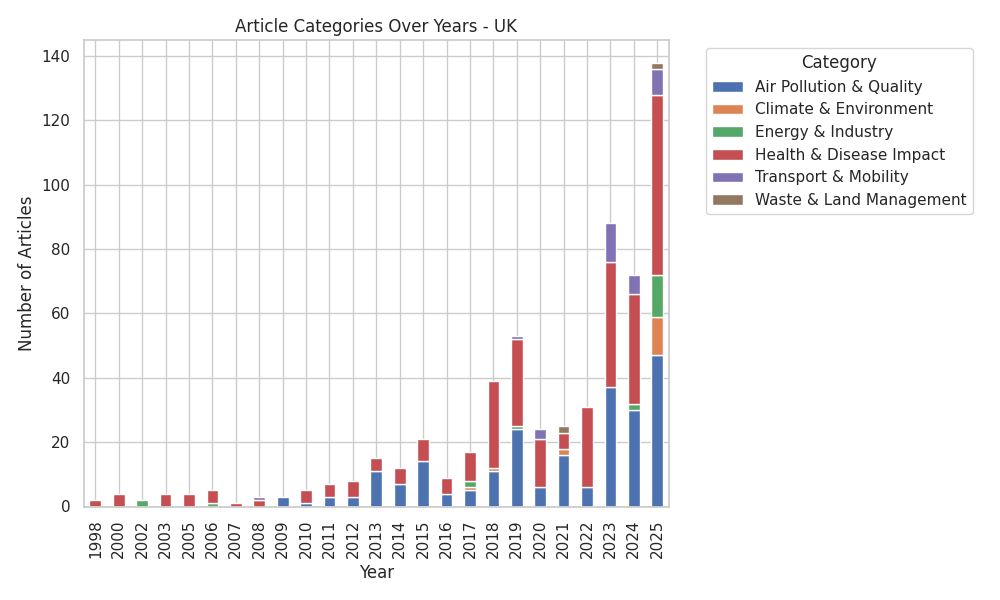
\includegraphics[width=0.5\linewidth]{uk_stacked_bar (1).png}
    \caption{Article categories over the years - United Kingdom}
    \label{fig:placeholder}
\end{figure}

\begin{figure}
    \centering
    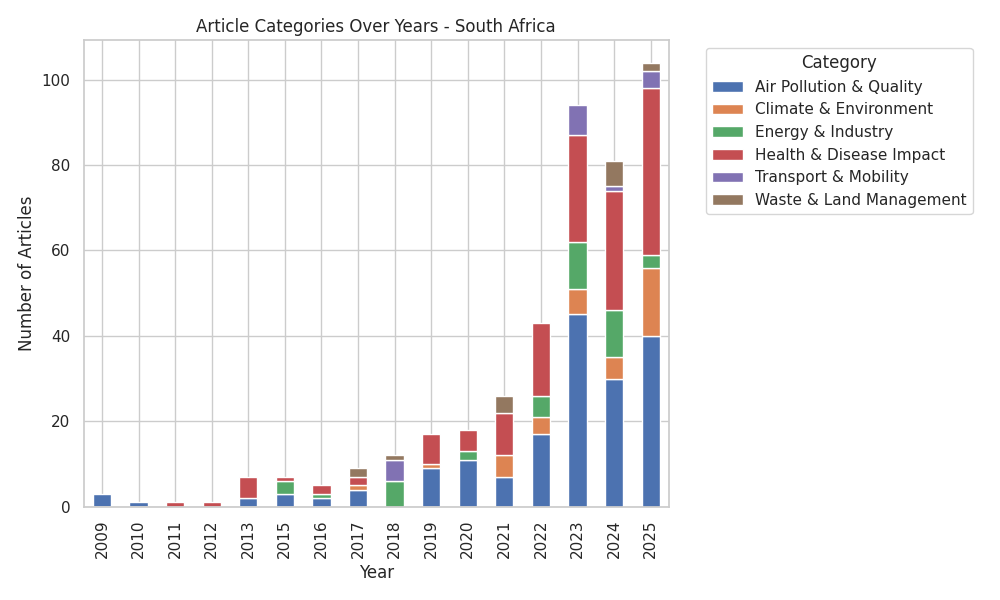
\includegraphics[width=0.5\linewidth]{south_africa_stacked_bar (1).png}
    \caption{Article categories over the years - South Africa}
    \label{fig:placeholder}
\end{figure}

\begin{figure}
    \centering
    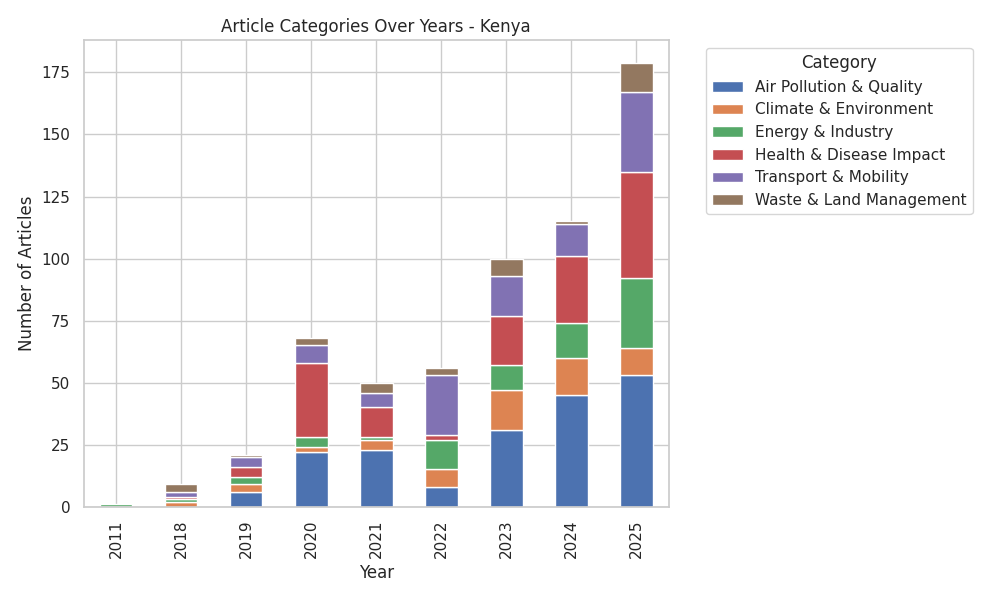
\includegraphics[width=0.5\linewidth]{kenya_stacked_bar (1).png}
    \caption{Article categories over the years - Kenya}
    \label{fig:placeholder}
\end{figure}

We also categorized published articles based on what they addressed under the topic of air quality and health. Our broad categorization included transport, and 

Transport and mobility in Kenya accounted for a higher percentage of articles due to the surge in electric bus and motorbike initiatives, which make up a significant portion of the country's transportation. This is also true for household energy, with the promotion of LPG (liquid petroleum gas) cookers and multiple initiatives aimed at reducing the use of biofuels in the country. 

\begin{figure}
    \centering
    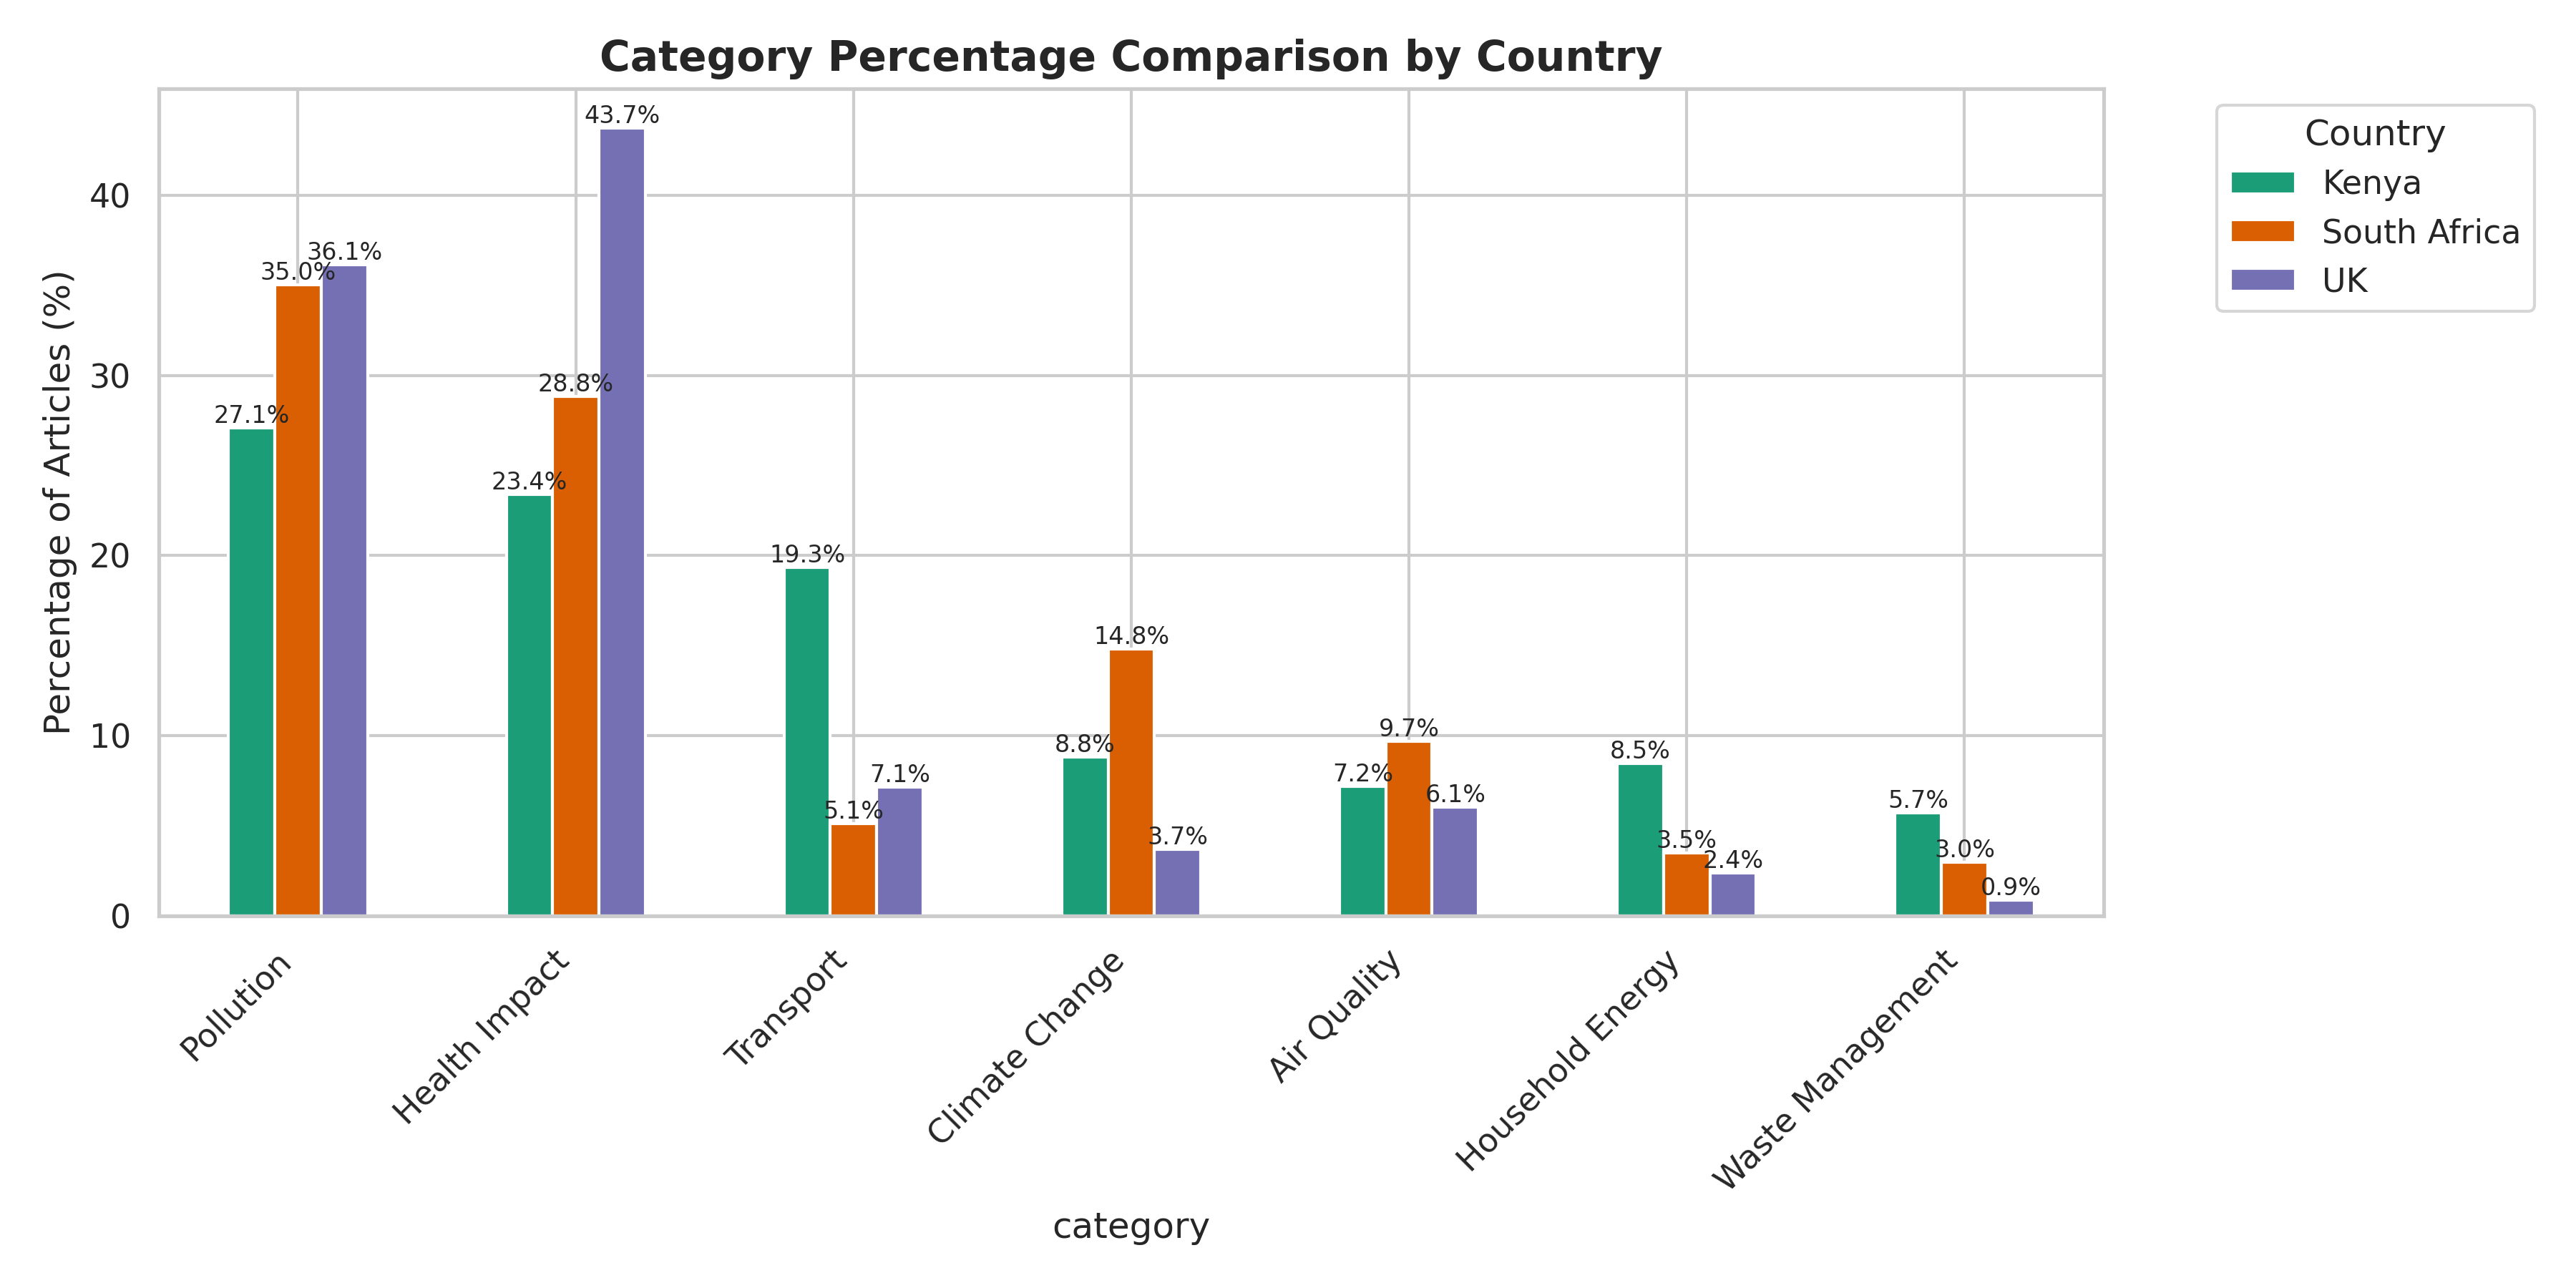
\includegraphics[width=0.5\linewidth]{category_percentage_comparison.png}
    \caption{Comparison of categories in the countries}
    \label{fig:placeholder}
\end{figure}


\section{Discussion}
Radio is the most common form of media exposure for both women and men in Kenya, followed by the newspaper and then television. More men than women are overall exposed to all three forms regularly. A higher percentage of men than women have daily internet access. Such statistics play a crucial role in regions where women continue to assume traditional roles and spend the majority of their time on household chores, including cooking. They are the ones who use biofuels and are impacted by the effects. They would benefit from better communication of the results of the impact of poor air quality.

Publications are the mode of communication of researchers. Through them, we can see the available data for use in different regions, the tools and techniques used to integrate them, and the highlighted challenges that prevent their integration.  

In resource-constrained and thus data-sparse regions, it would be beneficial to pull resources and data. This would undoubtedly help reduce fragmentation, fill in gaps, and even contribute to historical data. It does build up to a larger conversation about data sharing practices, licenses, open data, and more.  

Are we underestimating the magnitude of pollution in the regions due to these biases? 

The limitation of the studies to smaller cohorts failing to give true perspective of matters or issues. And with the knowledge that private sectors are less bureaucratic but also (this is not based on any evidence).



\end{document}
